\documentclass[journal]{IEEEtran}
\usepackage{Geoff,graphicx,amsmath,subfig}
\newenvironment{myalign}{\par\nobreak\noindent\align}{\endalign}

\title{Statement of Research Interests}
\author{Geoffrey Iyer} \date{}
\begin{document}
\maketitle
\vspace*{-2cm}

%%%%%%%%%%%%%%%%%%%%%%%%%%%%%%%%%%%%%%%%%%%%%%%%%%
% Todo list: Final review
%%%%%%%%%%%%%%%%%%%%%%%%%%%%%%%%%%%%%%%%%%%%%%%%%%

\section{Introduction}
\label{sec:intro}

The main focus of my research is in multimodal data and data fusion. With the
increasing availability of data we often come upon multiple datasets, derived
from different sensors, that describe the same object or phenomenon. We call the
sensors \emph{modalities}, and because each modality represents some new degrees
of freedom, it is generally desirable to use more modalities rather than fewer.
For example, in the area of speech recognition researchers have found that
integrating the audio data with a video of the speaker results in a much more
accurate classification \cite{Potamianos03}. However, correctly processing a
multimodal dataset is not a simple task \cite{lahat:hal-01062366}. The main
difficulty in multimodality lies in finding a way to coordinate information that
is represented in different formats. In the current state-of-the-art, most
multimodal algorithms apply only to very specific types of data, and are
therefore only useful for a small class of problems. Therefore it is desirable
to produce an algorithm that is robust to many different types of input
data. This has been the motivation of my PhD research.

The direction of my research group is heavily based around the representation of
the data as a weighted graph and the information we can glean from the
associated graph Laplcian (section \ref{sec:GraphRep}). The graph representation
allows us to discard the specifics of each data format and create objects that
can be directly compared. From this, we created an algorithm segments a
multimodal dataset under the assumption that the data is co-registered (the
modalities share a common indexing).  In section \ref{sec:CoReg} we give a brief
overview of the work done, and the full version can be found in \cite{Iyer2017}.
Our second algorithm is a work in progess, and is the focus of the remainder of
my PhD. Here we focus on eliminating the coregistration assumption by
introducing a matching process based on the geometry of each dataset. An
overview of the work done here can be found in section
\ref{sec:GraphMatch}. Finally, in section \ref{sec:relevance} we outline the
relevance to the Anticipatory Analysis project.

% One way of addressing multimodality in a general sense is to view each set of
% data as a manifold in some $\R$-space. We then look to form comparisons
% between the different manifolds via topological/geometric qualities of the
% sets. Since each manifold is derived from the same underlying source, we
% expect that there is enough commonality between the sets to obtain a
% reasonable correspondence this way. Some examples of this approach can be
% found in \cite{Yeh14}, where the authors use Canonical Correlation Analysis to
% compare the sets, and in \cite{Wang:2013:MAP:2540128.2540378, Tuia2016}, both
% of which use graph-based methods to perform feature extraction, then make
% comparisons on the feature level.  In this project, we aim to create an
% algorithm to compare manifolds using graph matching techniques. Each dataset
% will be represented as a weighted graph (similar to
% \cite{Wang:2013:MAP:2540128.2540378, Tuia2016}), which we will then use for
% the remainder of the algorithm. The advantage of the graph representation is
% its robustness to deformation. The weights are based only on the similarity
% between graph nodes, so they are invariant under conformal mappings, and
% relatively resilient towards continuous change. We will then solve a
% registration problem, matching nodes between the two graphs in a manner that
% preserves the graph geometry. This match can then be lifted to the original
% datasets, giving us a tool with which compare the different modalities. In the
% current state of the project, we have created a preliminary implementation of
% a graph matching algorithm based on the work in \cite{Umeyama1988,Knossow2009}
% and have completed a few experiments to test (a) the quality of the match, and
% (b) our ability to use this match to solve interesting problems involving more
% than one dataset.

% The rest of this paper is organized as follows. In section \ref{sec:method} we
% present the theory behind our algorithm. Section \ref{subsec:WGMP} defines the
% weighted graph matching problem (WGMP) in detail. We then reprise the results
% of \cite{Umeyama1988,Knossow2009} in \ref{subsec:graphLaplacian}, followed by
% our own improvements in \ref{subsec:hierarchical}. In section
% \ref{sec:experiment} we show the efficacy of our algorithm on an example
% dataset, followed by an application of our graph matching towards a change
% detection problem. Finally, in \ref{sec:futurework} we expound upon the
% direction of this project, explaining our main goal, as well as several
% additional contributions that we aim to make.

%%%%%%%%%%%%%%%%%%%%%%%%%%%%%%%%%%%%%%%%%%%%%%%%%%%%%%%%%%%%
% I didn't cite these in the intro and I feel bad about it:
%
% try citing \cite{Umeyama1988,Knossow2009,211474,Vogelstein2015,NIPS2013_4925}
% \cite{4641936} has it's own algorithm, plus citations to a lot of nice stuff.
% \cite{doi:10.1142/S0218001404003228} is a survey article of applications of
% graph matching to real problems.
%%%%%%%%%%%%%%%%%%%%%%%%%%%%%%%%%%%%%%%%%%%%%%%%%%%%%%%%%%%%
\section{Graph Representation}
\label{sec:GraphRep}
For notation, we label our different modalities as $X^1,X^2,\ldots,X^k$.  We
represent each $X^{\ell}$ using an undirected graph $G^\ell =
(V^\ell,E^\ell)$. The nodes $v^\ell_i\in V^\ell$ of the graph correspond to
elements of $X$, and we give each edge $e^\ell_{ij}$ a \emph{weight}
$w^\ell_{ij}\geq 0$ representing the similarity between nodes
$v^\ell_i, v^\ell_j$, where large weights correspond to similar nodes, and small
weights to dissimilar nodes. This gives rise to a \emph{similarity matrix} (also
called the \emph{weight matrix})
\begin{myalign}
  W^\ell = \left(w^\ell_{ij}\right)_{i,j=1}^n.
\end{myalign}
There are many different notions of ``similarity'' in the literature, and each
has its own merits. In particular, it is common to use an RBF kernel
\begin{myalign}
  w_{ij} = \text{exp}\left(-\norm{v_i -v_j} / \sigma \right),
\end{myalign}
where the details of the choice of norm and scaling parameter $\sigma$ depend on
the specific application.

Given a similarity matrix $W$, we then define the \emph{normalized graph
  Laplacian}.  For each node $v_i\in V$, define the \emph{degree} of the node
$d_i = \sum_j w_{ij}.$ Intuitively, the degree represents the strength of a
node. Let $D$ be the diagonal matrix with $d_i$ as the $i$-th diagonal entry. We
then define the normalized graph Laplacian.
\begin{myalign}
  L_{sym} = I - D^{-1/2}WD^{-1/2}.
\end{myalign}
For a thorough explanation of the properties of the graph Laplacian, see
\cite{Mohar91}. Here we use the fact that the eigenvectors of the graph
Laplacian solve the \emph{relaxed Graph min-cut problem}
\begin{myalign}
  \text{argmin}_{Q^TQ = I}\text{Tr}\left(Q^TL_{sym}Q\right),
\end{myalign}
and can be considered as features extracted from the dataset.
\vspace*{-0.5cm}
\subsection{Nystrom Extension}
\label{subsec:Nystrom}
Calculating the full graph Laplacian is computationally intensive, as the matrix
contains $n^2$ entries. Instead we use Nystr\"{o}m's extension to find
approximate eigenvalues and eigenvectors with a heavily reduced computation time
\cite{Fowlkes04}.

Let $X$ denote the set of nodes of the complete weighted graph. We choose a
subset $A\subset X$ of ``landmark nodes'', and have $B$ its complement. Up to a
permutation of nodes, we can write the weight matrix as
\begin{align}
  W = \begin{pmatrix} W_{AA} & W_{AB} \\ W_{BA} & W_{BB}
  \end{pmatrix},
\end{align}
where the matrix $W_{AB} = W_{BA}^T$ consists of weights between nodes in $A$
and nodes in $B$, $W_{AA}$ consists of weights between pairs of nodes in $A$,
and $W_{BB}$ consists of weights between pairs of nodes in $B$. Nystr\"{o}m's
extension approximates $W$ as
\begin{align}
  W \approx \begin{pmatrix} W_{AA} \\ W_{BA} \end{pmatrix}
  W_{AA}^{-1} \begin{pmatrix} W_{AA} & W_{AB}\end{pmatrix}.
\end{align}
In fact, it is possible to find $\abs{A}$ approximate eigenvectors of $W$ using
only the matrices $W_{AA},W_{AB}$. This results in a significant reduction in
computation time, as we compute and store matrices of size at most
$\abs{A}\times\abs{X}$, rather than $\abs{X}\times\abs{X}$.

\section{Feature Extraction and Segmentation on Multimodal Datasets}
\label{sec:CoReg}
In this section we assume that our datasets are \emph{co-registered}. That is,
the sets share a common indexing. Let $n = \abs{X^1} = \cdots = \abs{X^k}$, and
form the concatenated set
\begin{myalign}
  X = (X^1, \ldots, X^k) \subseteq \R^{n\times (dim_1+\cdots+dim_k)}.
\end{myalign}
to define the similarity matrix $W$, we must somehow compare the individual
$X^1,\ldots,X^k$. We do this by comparing distances between points in each
dataset. For $\ell = 1,\ldots,k$ define the scaling factor
\begin{myalign}
  \lambda_\ell = \text{stdev}\left(\norm{x_i^\ell-x_j^\ell}_{L^2}\; :\;1\leq i,j
    \leq n\right)
\end{myalign}
We then define the weight matrix $W$ by
\begin{myalign}
  w_{ij} &= \text{exp}\left(-\max\left(\frac{\norm{x^\ell_i -
          x^\ell_j}_{L^2}}{\lambda_\ell}\; : \; 1\leq \ell \leq k\right)\right).
\end{myalign}
We specifically choose to use the maximum of the individual measurements to
emphasize the unique information that each dataset brings. With this norm, two
data points $x_i,x_j$ are considered similar only when they are similar in every
modality.

Based on section \ref{sec:GraphRep}, we can extract features from $X$ via graph
Laplacian theory applied to the matrix $W$. From these features we then apply
segmentation algorithms to the feature set to obtain the final output. One
simple and straightfoward segmentation method is \emph{Spectral Clustering}, in
which we apply $k$-means to the set of features. We also implemented a
semisupervised graph MBO method \cite{MERKURJEV201429}, in which we minimize a
Ginzburg-Landau energy
\begin{myalign}\label{eqn:GinzburgLandauEnergy}
  E(u) &= \epsilon \cdot \text{Tr}\left(u^TL_{sym} u\right) +
  \frac{1}{\epsilon}\sum_i W(u_i) \\ &+ \sum_i
  \frac{\mu}{2}\lambda(x_i)\norm{u_i - \hat{u}_i}^2_{L_2}.
\end{myalign}
by iterative diffusion and thresholding. In figure \ref{fig:DFC}, we show the
results of our algorithm applied to the Data Fusion Contest 2015 dataset, which
consists of both lidar and RGB satellite images. Note that in the example
feature vectors \ref{fig:DFCevec01} \ref{fig:DFCevec02}, objects are separated
based both on color and on elevation. These separations are then reflected in
the final segmentation result.
% \subsection{Semisupervised Graph MBO}\label{subsec:MBO}
% To then segment our dataset we minimize a Ginzburg-Landau energy with a
% semisupervised term \cite{Garcia2014,Merkurjev13,MERKURJEV201429}. Have $u$ an
% $n \times m$ assignment matrix with
% \begin{myalign}
%   u_{ij} \geq 0 \; \forall i,j,\;\; \sum_{j=1}^m u_{ij} = 1.
% \end{myalign}
% The final output of the algorithm will be a matrix $u$ where each value is
% either $0$ or $1$. The energy we minimize is
% \begin{myalign}\label{eqn:GinzburgLandauEnergy}
%   E(u) &= \epsilon \cdot \text{Tr}\left(u^TL_{sym} u\right) +
%   \frac{1}{\epsilon}\sum_i W(u_i) \nonumber \\ &+ \sum_i
%   \frac{\mu}{2}\lambda(x_i)\norm{u_i - \hat{u}_i}^2_{L_2}.
% \end{myalign}
% The first term is the graph cut energy, similar to (\ref{eqn:NCut}). The
% second term is the multiwell potential
% $ W(u_i) = \prod_{k=1}^{m}\frac{1}{4}\norm{u_i - e_k}_{L_1}^2$ where $e_k$ is
% the $k$-th standard basis vector.  The last term includes the fidelity, where
% $\hat{u}$ represents the semisupervised input,
% \begin{myalign}
%   \lambda(x_i) = \begin{cases} 1 \quad \text{if $x_i$ is part of fidelity input}\\
%     0 \quad \text{else}
%   \end{cases},
% \end{myalign}

% We minimize this via iteritive diffusion and thresholding. If $u^{n}$
% represents the $n$-th iterate, then to calculate $u^{n+1}$ we first diffuse
% \begin{myalign}\label{eqn:diffusion}
%   \frac{u^{n+\frac{1}{2}}-u^n}{dt} = -L_{sym} u^n - \mu \lambda(x) (u^n -
%   \hat{u}).
% \end{myalign}
% Then threshold each row
% \begin{myalign}\label{eqn:threshold}
%   u_i^{n+1} = e_r \quad \text{where }r =
%   \text{argmax}_ju_{ij}^{n+\frac{1}{2}}.
% \end{myalign}
% The diffusion calculation can be done very efficiently by using the
% eigendecomposition of $L_{sym}$ (the feature vectors described in
% (\ref{eqn:relaxedNCut})). If we write change coordinates to the eigenbasis,
% then the diffusion step reduces to solving for coefficients
% \begin{myalign}
%   a_k^{n+1} = (1 - dt \cdot \lambda_k)\cdot a_k^n - dt\cdot d_k^n.
% \end{myalign}
% where $\lambda_k$ is the $k$-th eigenvalue of $L_{sym}$, in ascending order.
\begin{figure}
  \centering \subfloat[RGB Data]{%
    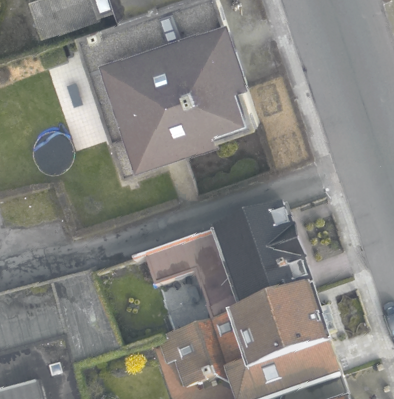
\includegraphics[width=0.48\columnwidth]{./Images/DFC2015/optical.png}%
    \label{fig:DFCoptical}%
  }%
  \hfill \subfloat[Lidar Data]{%
    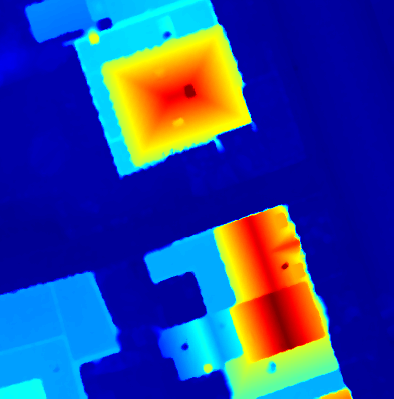
\includegraphics[width=0.48\columnwidth]{./Images/DFC2015/lidarColor.png}%
    \label{fig:DFClidar}%
  }%
  \hfill \subfloat[Example Eigenvector 1]{%
    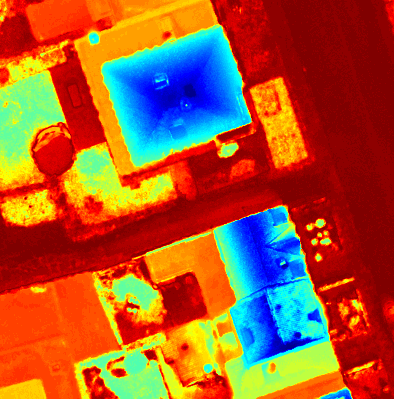
\includegraphics[width=0.48\columnwidth]{./Images/DFC2015/evec01.png}%
    \label{fig:DFCevec01}%
  }%
  \hfill \subfloat[Example Eigenvector 2]{%
    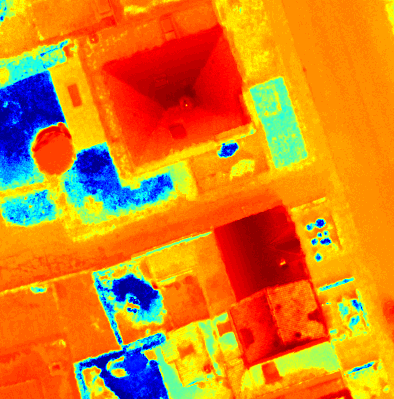
\includegraphics[width=0.48\columnwidth]{./Images/DFC2015/evec02.png}%
    \label{fig:DFCevec02}%
  }%
  \hfill %
  \subfloat[Spec. Clust. (Unsupervised)]{%
    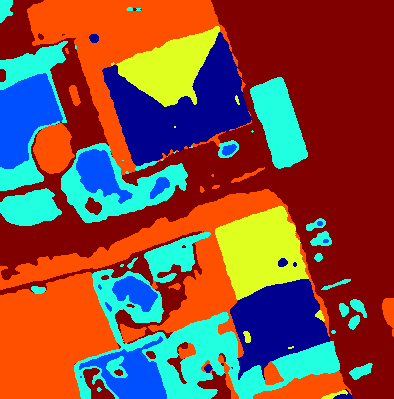
\includegraphics[width=0.48\columnwidth]{./Images/DFC2015/specClust.png}%
    \label{fig:DFCSpecClust}%
  }%
  \hfill \subfloat[MBO (Semisupervised)]{%
    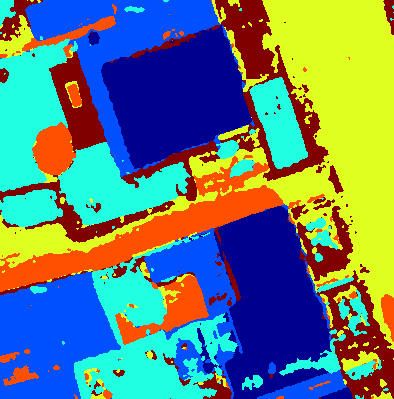
\includegraphics[width=0.48\columnwidth]{./Images/DFC2015/MBO.png}%
    \label{fig:DFCMBO}%
  }%
  \caption{DFC2015 Data and Results}
  \label{fig:DFC}
\end{figure}
\section{Graph Matching}
\label{sec:GraphMatch}
% Given two datasets $X,Y$, we will define the corresponding undirected,
% weighted graphs $G = (X,W_X)$, $H = (Y,W_Y)$. Here the nodes of $G$
% (resp. $H$) correspond to the points in $X$ (resp. $Y$). The weight matrix
% $W_X$ has size $\abs{X}\times\abs{X}$, and the value $W_X(i,j)$ represents the
% similarity between nodes $X(i),X(j)$ (and similar for $W_Y$). There are many
% possible definitions of $W_X$ in the literature, but the most common involve a
% RBF kernel, as we use in our experiments (section \ref{sec:experiment},
% equation \ref{eqn:graphweight}).
The above algorithm gives an effective way of comparing multiple modalities, but
for some problems we cannot assume our sets are coregistered. To address this
problem, we look to create our own registration by using the geometry of the
data. One common formulation of this problem is the Weighted Graph Matching
Problem (WGMP), described below.

Let $G = (X,W_X)$, $H = (Y,W_Y)$ be undirected, weighted graphs. Here $X, Y$
represent the nodes of $G, H$ (respectively), and $W_X,W_Y$ are the
corresponding matrix of edge weights. For convenience of notation we will assume
$\abs{X} = \abs{Y} = N$. The extension to the general case is quite
straightforward. The goal of the WGMP is to find a bijection $\rho:X \to Y$ that
minimizes the squared difference of edge weights. Phrased in terms of matrices,
our minimization problem becomes
\begin{myalign}
  \label{eqn:WGMPperm} \text{argmin}_{P\text{ a permutation
      matrix}}\norm{PW_XP^T - W_Y}^2_F.
\end{myalign}
Finding an exact solution to this problem is NP-Hard \cite{Arvind2012}. Instead,
we look for an approximate solution via the methods presented in
\cite{Umeyama1988}. Specifically, we relax the problem and search for an
orthogonal matrix.
\begin{myalign}
  \label{eqn:WGMPorthog} Q^* = \text{argmin}_{QQ^T=I}\norm{QW_XQ^T - W_Y}^2_F.
\end{myalign}
This problem was solved theoretically in \cite{Umeyama1988} using eigenvectors
of the graph Laplacian. Let $L_X = U_X \Lambda_X U_x^t$, be the
eigendecomposition of the graph Laplacian of $X$, and similarly have
$L_Y = U_Y \Lambda_Y U_Y^T$. Then the spectral graph matching theorem from
\cite{Umeyama1988} states that if each $L_x,L_y$ has distinct eigenvalues, the
optimal $Q$ from ($\ref{eqn:WGMPorthog}$) is given by
\begin{myalign}
  \label{eqn:WGMPorthogsolution} Q^* = U_Y^T S U_X,
\end{myalign}
where $S$ is a diagonal matrix with values $\pm 1$ to account for the sign
ambiguity in eigenvectors. In the current state of our project, we are using a
semi-supervised method to determine $S$. If we know of even one preexisting
match between the nodes in $X, Y$, we can use this to compare eigenvectors
$U_X,U_Y$ and add the appropriate signs.
% The calculation of $S$ can be rather frustrating, as there are $2^N$
% possibilities for this matrix. In \cite{Umeyama1988} the authors omit $S$
% entirely by replacing $U_k$ with $\abs{U_k}$ in equation
% \ref{eqn:WGMPorthogsolution}. In \cite{Knossow2009} the authors determine $S$
% by looking at the histograms of the columns of $U_k$ (which are invariant
% under permutation) and adding $\pm$ according to the best fit.

Note that if we ignore the sign ambiguity (assume $S = I$), then the solution
reduces to $Q^* = U_Y^T U_X$. In other words, we measure the similarity between
graph nodes by taking inner products in the eigenvector feature space.  To
complete our approximate solution to the WGMP, we use the matrix $Q^*$ to find a
matching
\begin{myalign}
  \rho: \{1,2,\ldots,N\} \to \{1,2,\ldots,N\}.
\end{myalign}
% In the original formulation of the WGMP \ref{eqn:WGMPperm}, an entry of $1$ at
% position $(i,j)$ in the permutation matrix $P$ represents a match between node
% $i$ of $Y$ with node $j$ of $X$. In the relaxed version of the problem,
The task of converting $Q^*$ to a permutation $\rho$ is easily solved using the
Hungarian algorithm, which in $O(N^3)$ time finds the matching $\rho$ that
maximizes the sum of similarity scores
\begin{myalign}
  \sum_{i=1}^N Q^*(i,\rho(i)).
\end{myalign}

% In practice, one often does not use every eigenvector of $L_X,L_Y$ in the
% calculation of $Q$. Rather, we choose a number $K \ll N$, and let $U_k$ be the
% $N\times K$ matrix where the columns are the eigenvectors corresponding to the
% $K$ smallest eigenvalues. Heuristically, the columns of $U_k$ represent
% features extracted from the original graph, and the size of the corresponding
% eigenvalues represents the strength of each particular feature. If we then
% assume that the sign ambiguity has been dealt with (so that $S = I$), then
% $Q^* = U_YU_X^t$.  That is, $Q^*(i,j)$ is the dot product of row $i$ of $U_Y$
% with row $j$ of $U_X$. So we are determining match strength by comparing the
% images of our data in this new feature space. In doing this, we can also
% handle the case where $\abs{X}\neq\abs{Y}$. If we chose
% $K \leq \min(\abs{X},\abs{Y})$, then formula (\ref{eqn:WGMPorthogsolution})
% will still hold, and $Q^{*}$ will be an $\abs{Y} \times \abs{X}$ matrix
% representing the node similarities.

%%%%%%%%%%%%%%%%%%%%%%%%%%% 
% This was a good little bit on the heuristics, but I don't know where to put
% it.

% Heuristically, the columns of $U_k$ (the eigenvectors of $L_k$) represent
% features extracted from the original graph, and the rows of $U_k$ give the
% images of each graph node in this new feature space. If we assume that the
% sign ambiguity has been dealt with (so that $S = I$), then $Q^* =
% U_YU_X^t$. That is, $Q^*(i,j)$ is the dot product of row $i$ of $U_Y$ with row
% $j$ of $U_X$

% In practice, we don't use all N eigenvectors. That's CRAZY!
%%%%%%%%%%%%%%%%%%%%%%%%%%% 

%%%%%%%%%%%%%%%%%%%%%%%%%%%
% The benefits of Graph Matching. Should go somewhere

% Benefits of Graph Matching
% \begin{enumerate}
% \item A precise number representing similarity between nodes gives us many
%   options.
%   \begin{itemize}
%   \item Thresholding
%   \item Many-to-many matching
%   \item Hierarchical matching
%   \end{itemize}
% \item Easy extension to the case $\abs{G_1}\neq\abs{G_2}$.
% \item Robust to many continuous deformations.
%   \begin{itemize}
%   \item scaling, shifts, rotations, etc.
%   \end{itemize}
% \end{enumerate}
%%%%%%%%%%%%%%%%%%%%%%%%%%
\vspace*{-0.5cm}
\subsection{Hierarchical graph matching}
\label{subsec:hierarchical}

The advantage of the Hungarian algorithm is that it results in the optimal
one-to-one matching based on the input data, but the $O(N^3)$ runtime is an
undesirable feature. To solve this we introduce a hierarchical structure to the
above algorithm. Specifically, we create smaller ``coarsified'' graphs
$\tilde{G},\tilde{H}$ of size $M \ll N$. These $\tilde{G},\tilde{H}$ should
represent the same geometric structure as $G,H$, but with many fewer nodes. We
then graph matching algorithm on $\tilde{G},\tilde{H}$, giving us a match on the
coarse level. To lift this to a match between $G,H$, for each match $i \to j$ in
the coarse graphs we run our graph matching algorithm between the corresponding
clusters in the original graph. So in total, we create 1 match of size $M$, and
$M$ matches of size $\frac{N}{M}$, which significantly improves the runtime. In
practice, our prototype code can handle sets of size up to $N = 100,000$.  In
theory, we could achieve an even better runtime via better optimizations and
parallel processing. We could also speed up the matching process by performing
multiple coarsification steps, and iteratively matching the graphs on
increasingly fine levels. However, this would give dimishing returns with each
added layer, as well as create some issues with error propagation.
\vspace*{-0.5cm}
\subsection{Example graph matching}
\label{subsec:experiment}
%%%%%%%%%%%%%%%%%%%%%%%%%%%%%%%%%%%%%%%%%%%%%%%%
% If we want an example Hungarian algorithm I have it here
%
% Say we have $N=6$ and calculated:
% \[Q^* = \begin{pmatrix} -0.1629 & -0.1711 & -0.1703 & 0.3426 & 0.3717 &
%     -0.2100\\ -0.1647 & -0.1662 & -0.1677 & 0.2966 & 0.3192 & -0.1172\\
%     -0.1660 & -0.1653 & -0.1657 & -0.1477 & -0.1861 & 0.8308\\ -0.4579 &
%     0.6860 & 0.2665 & -0.1787 & -0.1480 & -0.1678\\ 0.4939 & -0.1039 & 0.1196
%     & -0.6689 & 0.3080 &
%     -0.1486\\ 0.4577 & -0.0795 & 0.1176 & 0.3561 & -0.6647 & -0.1872\\
%   \end{pmatrix}\] Then
% \[P^* = \begin{pmatrix}
%     0&0&0&1&0&0\\
%     0&0&0&0&1&0\\
%     0&0&0&0&0&1\\
%     0&1&0&0&0&0\\
%     1&0&0&0&0&0\\
%     0&0&1&0&0&0\\
%   \end{pmatrix}\]
%
%%%%%%%%%%%%%%%%%%%%%%%%%%%%%%%%%%%%%%%%%%%%%%%%

Here we show the results of our graph matching algorithm on a synthetic dataset,
pictured in figure \ref{fig:graphmatchsynthetic}. The nodes of the
graphs $G,H$ are represented by 2-dimensional datasets $X,Y$, and the weight
matrices $W_X,W_Y$ are determined via an RBF kernel applied to the 2-norm.
\begin{myalign}
  E_X(i,j) = \norm{X(i) - X(j)} \\
  W_X(i,j) =
  -\text{exp}\left(\frac{E_X(i,j)}{\text{stdev}(E_X)}\right), \label{eqn:graphweight}
\end{myalign}
and similar for $W_Y$. The matching is then calculated using the hierarchical
algorithm in \ref{subsec:hierarchical}, with the match on the coarse level
shown in figures \ref{fig:CoarseMatchX1}, \ref{fig:CoarseMatchX2},
\ref{fig:CoarseMatchResult}. This example has datasets of size $N = 1500$, with
$M=50$, so that the coarsified data has size
$\abs{\tilde{X}} = \abs{\tilde{Y}} = 30$.

The purpose of this example is to show that the matching algorithm can recognize
the geometry of the data. Both sets $X,Y$ contain a tight cluster of points, as
well as longer line segment. In figures \ref{fig:CoarseMatchResult},
\ref{fig:GraphMatchResult}, we see the final result of the algorithm, where each
match is represented by a line connecting the two points in question. As we can
see in the figure, the algorithm successfully matches the objects based on their
shape, as we desired.

\begin{figure}
  \centering \subfloat[Dataset $X$]{%
    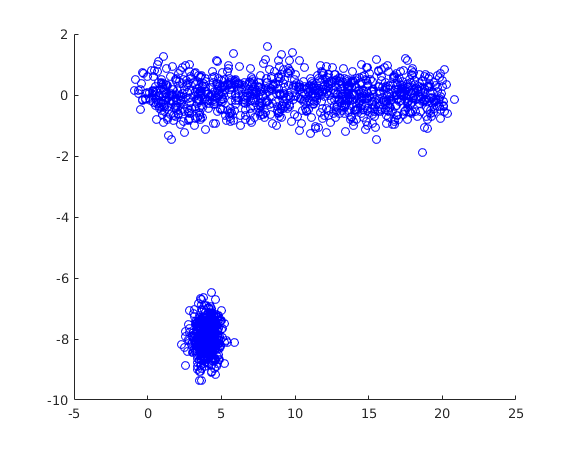
\includegraphics[width=0.47\columnwidth]{./Images/GraphMatch/Example1/X1.png}%
    \label{fig:GraphMatchX1}%
  }%
  \subfloat[Dataset $Y$]{%
    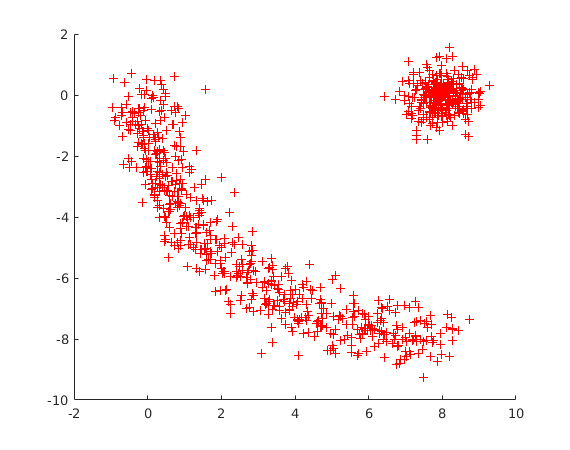
\includegraphics[width=0.47\columnwidth]{./Images/GraphMatch/Example1/X2.png}%
    \label{fig:GraphMatchX2}%
  }%
  \hfill%
  \subfloat[Coarsified data $\tilde{X}$]{%
    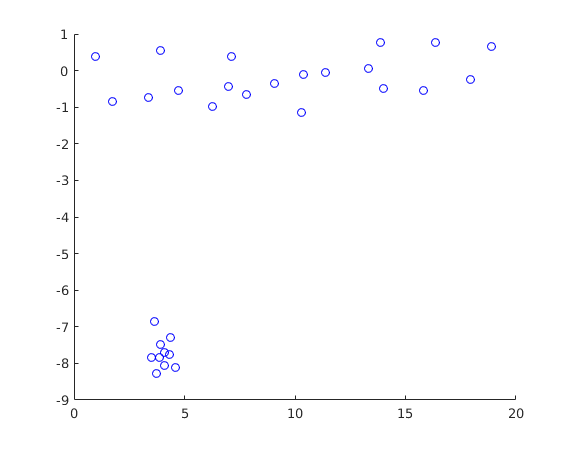
\includegraphics[width=0.47\columnwidth]{./Images/GraphMatch/Example1/coarseX1.png}%
    \label{fig:CoarseMatchX1}%
  }%
  \subfloat[Coarsified data $\tilde{Y}$]{%
    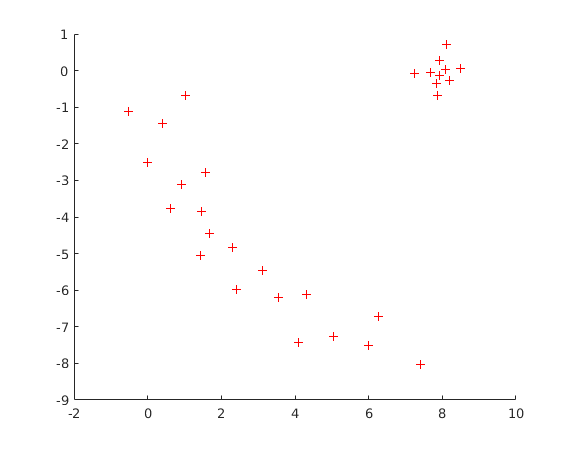
\includegraphics[width=0.47\columnwidth]{./Images/GraphMatch/Example1/coarseX2.png}%
    \label{fig:CoarseMatchX2}%
  }%
  \hfill %
  \subfloat[Graph match on coarse data]{%
    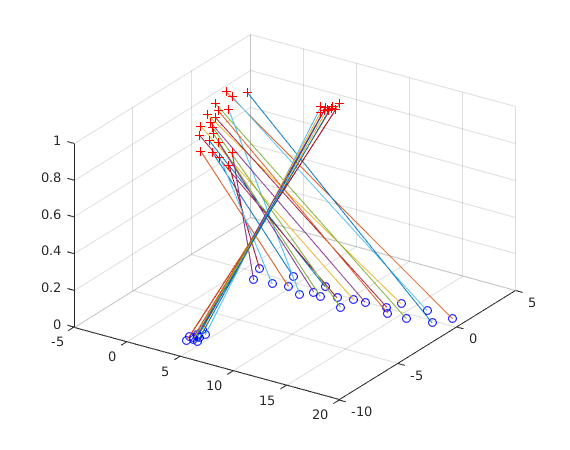
\includegraphics[width=0.47\columnwidth]{./Images/GraphMatch/Example1/coarseMatch.png}%
    \label{fig:CoarseMatchResult}%
  }%
  \subfloat[Hierarchical match result]{%
    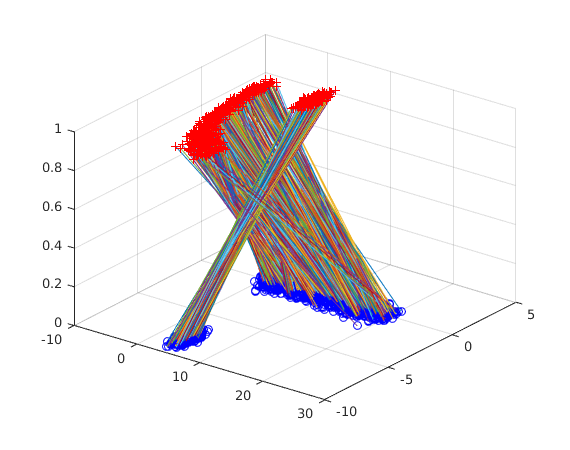
\includegraphics[width=0.47\columnwidth]{./Images/GraphMatch/Example1/graphmatch.png}%
    \label{fig:GraphMatchResult}%
  }%
  \caption{Example hierarchical matching on synthetic data}
  \label{fig:graphmatchsynthetic}
\end{figure}

% \subsection{Change detection using graph matching}

% There's a lot of stuff written for this what do I use?

% One possible application of graph matching is in change detection. Suppose
% that the sets $X,Y$ represent two images of the same scene, taken at different
% times. A direct comparison of $X$ to $Y$ is often not useful, as it is
% possible for individual pixels to change drastically while keeping the overall
% structure of the image the same. For example, if the images $X,Y$ were
% captured in different lighting, then the set $X-Y$ would show many ``false''
% changes. Instead, we turn to graph matching as a way to compare pixels between
% $X,Y$ in the context of the larger image.

% We will track the changes as follows: apply the matching algorithm to $X,Y$,
% and let $\rho:\{1,2,\ldots,N\} \to \{1,2,\ldots,N\}$ be the permutation of the
% indices corresponding to the match $X \to Y$. Then we measure the degree of
% change in the scene at pixel $i$ via the quantities
% \begin{myalign}
%   \text{Change in $X$ at pixel $i$} &= \norm{X(i) - X(\rho(i))} \\
%   \text{Change in $Y$ at pixel $i$} &= \norm{Y(\rho^{-1}(i)) - Y(i)}
% \end{myalign}

% As a first example, we apply the algorithm to a synthetic dataset, with the
% results shown in figure \ref{fig:changedetectsynthetic}. This data was
% constructed to mimic the above discussion, showing both a change in overall
% hue between images $X, Y$, as well as an actual structural change with the
% addition of a blue dot in $Y$. In this example, we consider the dot in $Y$ to
% be the only true ``change'' between the images. The change in hue represents
% some incidental affect in the data capture process, and should be ignored by
% the algorithm. Here, both images are size $80 \times 80$, for a total of
% $N = 6400$ pixels. The algorithm runs in roughly 10 seconds, and successfully
% highlights the dot in $Y$, as desired.

% \begin{figure}
%   \centering \subfloat[Image $X$]{%
%   \includegraphics[width=2.0in]{./Images/ChangeDetection/Example1/dataBefore.png}%
%   \label{fig:ChangeDetectionSyntheticX1}%
% }%
%   \hfill %
%   \subfloat[Image $Y$]{%
%   
\includegraphics[width=2.0in]{./Images/ChangeDetection/Example1/dataAfter.png}%
%   \label{fig:ChangeDetectionSyntheticX2}%
% }%
%   \hfill %
%   \subfloat[$\norm{Y(\rho^{-1}(i)) - Y(i)}$]{%
%   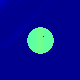
\includegraphics[width=2.0in]{./Images/ChangeDetection/Example1/normMap.png}%
%   \label{fig:ChangeDetectionSyntheticResult}%
% }%
%   \caption{Example change detection on synthetic data}
%   \label{fig:changedetectsynthetic}
% \end{figure}

% At this point in the project, we began working with real-world datasets. In
% figure \ref{fig:changedetectflood} we show a preliminary result of our
% algorithm on data from the 2010 Data Fusion Contest
% \cite{longbotham2012multi}. The dataset consists of remote sensing image of
% Gloucester, UK, taken both before (\ref{fig:ChangeDetectionX1}) and after
% (\ref{fig:ChangeDetectionX2}) a flood in the year 2000. The final result in
% figure \ref{fig:ChangeDetectionResult} is difficult to fully interpret, but it
% is encouraging to see the algorithm highlighting noteworthy shapes from the
% individual images. As we continue to improve our methods, we expect to see
% even more obvious results.

% % TODO I WANT A DIFFERENT SET OF IMAGES
% \begin{figure}
%   \centering \subfloat[Image $X$ (before flood)]{%
%   \includegraphics[width=2.0in]{./Images/ChangeDetection/Example2/dataBefore.png}%
%   \label{fig:ChangeDetectionX1}%
% }%
%   \hfill %
%   \subfloat[Image $Y$ (after flood)]{%
%   
\includegraphics[width=2.0in]{./Images/ChangeDetection/Example2/dataAfter.png}%
%   \label{fig:ChangeDetectionX2}%
% }%
%   \hfill %
%   \subfloat[$\norm{X(i) - X(\rho(i))}$]{%
%   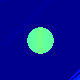
\includegraphics[width=2.0in]{./Images/ChangeDetection/Example2/normMap.png}%
%   \label{fig:ChangeDetectionResult}%
% }%
%   \caption{Example change detection on DFC 2010 data}
%   \label{fig:changedetectflood}
% \end{figure}

\section{Relevance to Anticipatory Analysis}
\label{sec:relevance}

Speaking in general terms, the Anticipatory Analysis project is deeply rooted in
multimodality. The scope of the data involved is very large both in size, as
well as in variety of formats, leading to many problems similar to the ones
addressed in my work. For example, timeseries data from a multiple different
sources can be considered to be coregistered based on observation time. We can
then apply the ideas from \ref{sec:CoReg} to extract feature vectors which can
be used for many different applications (including, but not limited to,
segmentation).

We could also apply our graph matching algorithm to such a dataset, then compare
the indexing given by graph matching against the natural coregistration
indexing. This would give us an idea of the level of redundancy between the
datasets. An example of this idea is shown in figure \ref{fig:ChangeDetect}.
Here we have two synthetic datasets, where the $x$-axis represents time of
observation (and is used to register the modalities), while the $y$-axis
represents the observed value. Looking at the input data (figure
\ref{fig:ChangeDetectData}, we see that the two modalities contain redundant
information for smaller $x$ values. Because of this, the graph match result is
very similar to the coregistration indexing for this region. Conversely,
the two modalities contain very different information for larger $x$ values. In
other words, the manifolds have different local geometries in this
area. Therefore the graph match does not compare well against the
coregistration. By applying a simple threshold to the observed match quality, we
are able to highlight the unique information contained in each modality, and
leave the redundant information untouched (figure \ref{fig:ChangeDetectResult}).

\begin{figure}
  \centering \subfloat[Input Data]{%
    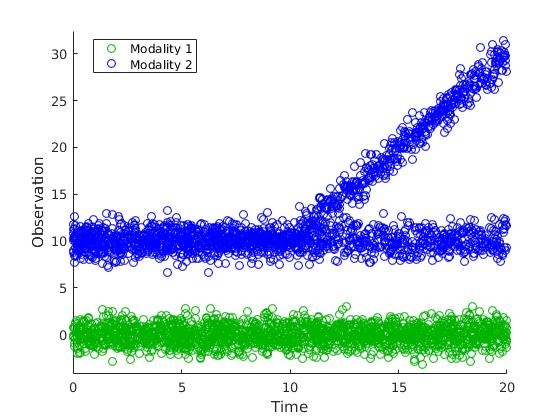
\includegraphics[width=0.70\columnwidth]{./Images/GraphMatch/SyntheticChange/InputData.jpg}%
    \label{fig:ChangeDetectData}%
  }%
  \hfill \subfloat[Poor Matches Highlighted]{%
    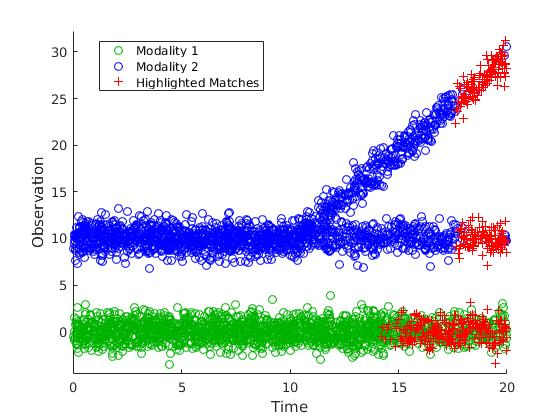
\includegraphics[width=0.70\columnwidth]{./Images/GraphMatch/SyntheticChange/BadMatches.jpg}%
    \label{fig:ChangeDetectResult}%
  }%
  \caption{Manifold comparison via graph match}
  \label{fig:ChangeDetect}
\end{figure}

Overall, graphs offer a powerful tool in comparing different modalities. By
reducing the input data to a set of similarities, we discard most of the
formatting specific to each dataset while still retaining the relevant
information. The resulting graph objects can then be compared directly, either
through some prior knowledge of registration, or via the geometry of each
set. Although this sounds intimidating from a computational standpoint, we have
access to powerful approximation tools that make our graph algorithms
competitive with the state of the art.
\vspace*{-0.5cm}
\bibliographystyle{unsrt} \bibliography{../../BibTex/research}
\end{document}
